现在我们有了地图和定位,终于可以进入我们的正题导航了。
我们使用的是Nav2导航框架,该项目力求以安全的方式让移动机器人从A点移动到B点。
Nav2也可以应用于其他应用,包括机器人导航,如下动态点跟踪,在这个过程中需要完成动态路径规划、
计算电机的速度、避免障碍、恢复行为。

Nav2使用行为树(详情见下一个章节)调用模块化服务器来完成一个动作。
动作可以是计算路径、控制力、恢复或任何其他与导航相关的操作。
服务器可以简单分为一大三小四个服务。
一大:
BT Navigator Server 导航行为树服务,
通过这个大的服务来进行下面三个小服务组织和调用。
\subsubsection{全局规划器}

Planner Server,规划服务器,(全局规划器)是Nav2中的核心模块之一,
它负责根据所选的命名法和算法规划机器人的全局路径,即从起始点到目标点的路径。
说白了就是在地图上找路。
他们通过全局代价地图global\_costmap,根据当前机器人的位置和目标位置,计算出从当前位置到目标位置的(时间或路程)最优路径。
路径规划算法有很多种,还有他们的优化版本。
这里,我们介绍两个最经典好用的算法:$Dijkstra$算法和$A*$算法
\paragraph{$Dijkstra$算法}
$Dijkstra$算法是一种最简单的广度优先的路径规划算法,它通过计算从起始点到其他所有点的最短路径,直到覆盖到终点。

\url{https://www.bilibili.com/video/BV19b4y1d7Hz/}


\subsubsection{控制器}
如果只有规划器会怎么样呢?

现在,登录你舍友的LOL账号,开一把排位晋级赛,在小地图上点击敌方基地。

\begin{figure}[H]
    \centering
    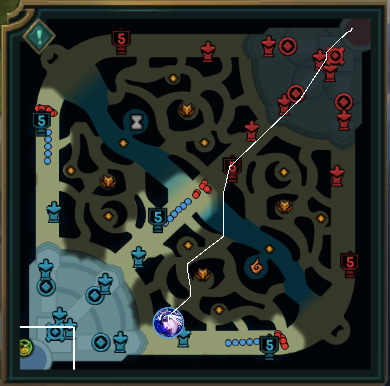
\includegraphics[width=0.8\textwidth]{./images/英雄联盟.png}
    \caption{全局路径(用A*算法根据障碍物(建筑)算出来的)}
\end{figure}
好的,一条全局导航路径生成出来了;好的,你的英雄沿着规划好的路径动起来了;好的,你被对面拿下一血并被队友问候全家。
这是为什么?因为敌方是动态的,他的位置不是事先知道的,事先知道的只有地图,而全局规划器只考虑了地图,未考虑动态障碍物。
局部规划器就是在你的视野里出现动态障碍物的时候,规划出一条道路绕开他,然后继续跟着全局路径走。

回到缺德地图,你这位车手就是局部规划器,缺德地图(全局规划器)只给大致的路线。
如何避让冲出来的小学生,掉头,超车,等红灯等都是车手(局部规划器)决定的。

控制器,在ROS 1中也被称为局部规划器,是我们跟随全局计算路径或完成局部任务的方法。控制器有权访问局部环境表达,
以尝试计算要跟随的基准路径的可行\textbf{控制工作}(即速度、加速度、角速度等)。许多控制器会将机器人向前投射到空间中,并在每次更新迭代时计算局部可行路径。
控制器可以被编写为具有以下功能的工具:
\begin{itemize}
    \item 跟随路径
    \item 使用里程计坐标系中的探测器,让机器人与充电站(桩)对接
    \item 登上电梯
    \item 与某个工具的接口交互
\end{itemize}
在Nav2中,控制器的一般任务是计算一个有效的\textbf{控制工作}以跟随全局规划路径。
然而,有多个控制器类和局部规划器类。
Nav2项目的目标就是所有控制器算法都可以作为此服务器中的插件,以用于一般研究和产业任务中。

常用的局部规划器有DWA,TEB等,我们使用的是TEB算法。